% IEEE standard conference template; to be used with:
%   spconf.sty  - LaTeX style file, and
%   IEEEbib.bst - IEEE bibliography style file.
% --------------------------------------------------------------------------

\documentclass[letterpaper]{article}
\usepackage{spconf,amsmath,amssymb,graphicx}
\usepackage{graphicx}
\usepackage{tabularx}
\usepackage[export]{adjustbox}


% Example definitions.
% --------------------
% nice symbols for real and complex numbers
\newcommand{\R}[0]{\mathbb{R}}
\newcommand{\C}[0]{\mathbb{C}}

% bold paragraph titles
\newcommand{\mypar}[1]{{\bf #1.}}

% Title.
% ------
\title{Parallel SAT Solving}
%
% Single address.
% ---------------
\name{Jan Eberhardt, Jakub Lichman}
\address{Department of Computer Science\\ ETH Zurich\\Zurich, Switzerland}

% For example:
% ------------
%\address{School\\
%		 Department\\
%		 Address}
%
% Two addresses (uncomment and modify for two-address case).
% ----------------------------------------------------------
%\twoauthors
%  {A. Author-one, B. Author-two\sthanks{Thanks to XYZ agency for funding.}}
%		 {School A-B\\
%		 Department A-B\\
%		 Address A-B}
%  {C. Author-three, D. Author-four\sthanks{The fourth author performed the work
%		 while at ...}}
%		 {School C-D\\
%		 Department C-D\\
%		 Address C-D}
%

\begin{document}
%\ninept
%
\maketitle
%

The hard page limit is 6 pages in this style. Do not reduce font size
or use other tricks to squeeze. This pdf is formatted in the American letter format, so the spacing may look a bit strange when printed out.

\begin{abstract}
Describe in concise words what you do, why you do it (not necessarily
in this order), and the main result.  The abstract has to be
self-contained and readable for a person in the general area. You
should write the abstract last.
\end{abstract}

\section{Introduction}\label{sec:intro}

\mypar{Motivation} Boolean satisfiability problem (SAT) belongs to the most important problems in program analysis, verification and other disciplines of theoretical computer science. It is particularly used in background of many applications, especially ones in the field of automated planning and scheduling, model checking(formal verification) and theorem proving. 

Last decade brought many improvements to SAT world in form of advanced heuristics, preprocessing and inprocessing techniques and data structures that allow efficient implementation of search space pruning. 

However, past 10 years were also rich on improvements in parallelism. Current trends in computer hardware design decreased performance per processing unit and pack more units on a single processor. It is caused by thermal wall which stopped further increase of clock speed. However, algorithms for SAT solving like DPLL and CDCL were invented before wide use of parallelism and therefore were designed for sequential execution. Since SAT is a NP-complete problem, we consider it the right candidate for running in parallel.

In our approach, we are trying to speed up SAT solving by running it on multiple cores with different techniques of search space partitioning. Final comparison is done between different parallel versions and sequential one. Parallel versions are mainly based on DPLL algorithm except the one which uses also CDCL, but locally. All algorithms are unlimited in number of cores they can run on. However, some scale better than the others. 

Experiments were run on the cluster where we were allowed to use at most 48 cores. Tests were taken from SATLIB - The Satisfiability Library \cite{cnf_website} and some were also created by our own random generator of formulas. Results show nice speedups in parallel versions against sequential one. However, parallel DPLL algorithm is still not able to outperform sequential CDCL. It shows how good CDCL actually is in comparison with DPLL. 

\mypar{Related work} Tomas Balyo et al. in their paper \cite{hordesat} propose HordeSat solver which can run up to 1024 cores and is based on CDCL algorithm. Their parallel approach is different from ours because it is portfolio based but with sign of search space partitioning. Most of the previous SAT solvers designed for computer clusters or grids use explicit search space partitioning. Examples of such solvers are GridSAT \cite{gridsat}, PMSAT \cite{pmsat} or ManySat \cite{manysat}. Paper that is probably closest to ours \cite{stealing} firstly introduced work stealing for dynamic load-balancing. 

\section{Background: Whatever the Background is}\label{sec:background}

\mypar{CNF} A \textit{boolean variable} is a variable that can be assigned either to \textit{true} or \textit{false}. A \textit{literal} of a boolean variable $x$ is considered to be in positive $x$ or negative  $\overline{x}$ form. A \textit{clause} is then disjunction (OR) of literals. A \textit{conjunctive normal form} (CNF) is a conjunction of such a clauses. CNF is usually represented by a number of variables and clauses.  However, measuring difficulty of CNF by these two factors is very inaccurate.  

\mypar{SAT} SAT solver is a program that is able to decide whether given formula is satisfiable. More formally, given formula $F$ is satisfiable \textit{iff} there \textit{exists} assignment of literals $\theta$ that makes whole formula (\textit{CNF}) true (\textit{satisfiable}). If there does not exits such an assignment then formula is \textit{unsatisfiable}. Furthermore, every SAT solver should be able in \textit{satisfiable} case provide valid assignments of literals as well. 

\mypar{History} First algorithm was develop in 1960 by Martin Davis and Hilary Putnam \cite{dp} for checking the validity of a first-order logic formula using a resolution-based decision procedure for propositional logic. Since Davis-Putnam algorithm was able to handle just valid formulas, more general approach for SAT solving was needed. In 1962 was developed new, complete algorithm that was able to handle all types of formulas. The algorithm is called \textit{DPLL} \cite{dpll} after Davis, Putnam, Logemann, and Loveland. It is backtracking-based search algorithm that still forms the basis for most efficient complete SAT solvers. Since DPLL invention, there were many algorithms proposed, which improved runtime of SAT solving significantly.
\begin{figure}
	\centering
	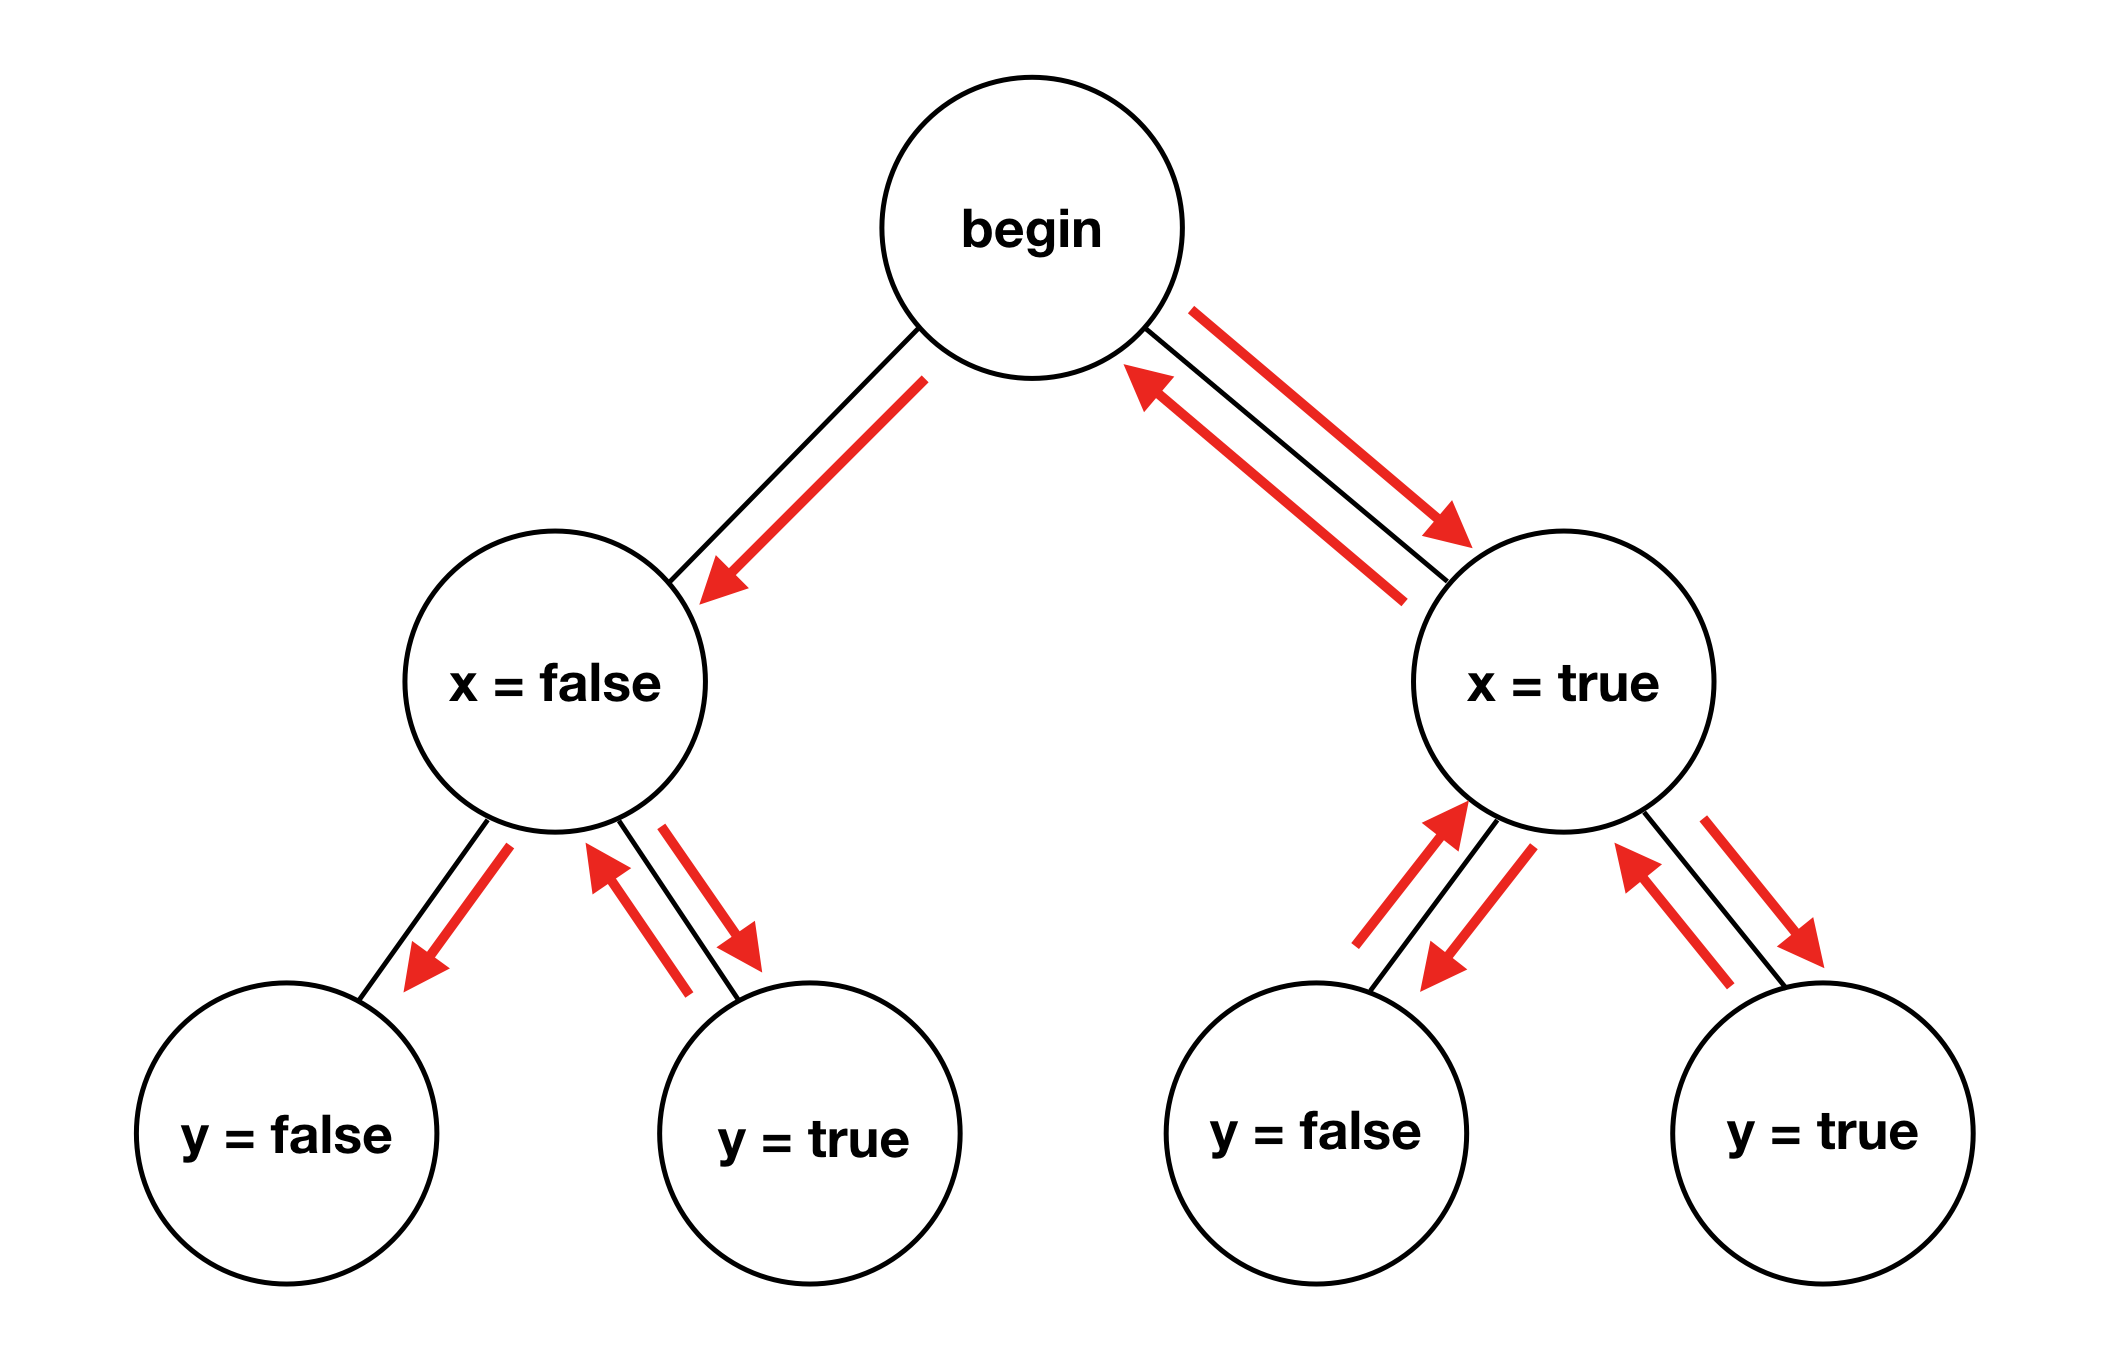
\includegraphics[width=\columnwidth]{figures/dpll-branching}
	\caption{The way how DPLL explores search space of CNF with two variables \textit{x} and \textit{y}.
		\label{fig:dpll-branching}}
\end{figure}

\mypar{DPLL} DPLL solves a SAT problem by modelling it as a decision tree, variables can either be assigned to \textit{true} or \textit{false}. In every step DPLL tries to find variables that are "automatically" assigned because of a previous decision,
if there are none it will pick a variable $v_i$ and assume a value for it.
If it later turns out that this decision was wrong it backtracks to that point and picks the negated assignment for variable $v_i$.

\mypar{CDCL} The algorithm performs as well as DPLL a depth-first search of the space of partial truth assignments. In addition to DPLL, Conflict-Driven Clause Learning (\textit{CDCL}) adopts a pruning technique called learning. While in DPLL we can solve same clauses multiple times, CDCL remembers them and in the next encounter avoids them. More formally, learning extracts and memorizes information from the previously searched space to prune the search in the future \cite{cdcl}. Learning is done by adding clauses to the existing clause database. Clauses are analyzed and stored whenever search reaches conflict state. If it cannot be resolved by backtracking then the formula is unsatisfiable. If all the variables are assigned and no conflict happened then the formula is satisfiable. \cite{hordesat}


\section{Parallelizing DPLL}\label{sec:parallel_dpll}

We decided to parallelize DPLL because it is a relatively simple backtracking algorithm and therefore it does not require any advanced communication.
Subtasks can be solved individually and therefore also on different nodes.

\mypar{DPLL Branches}
As introduced in Section \ref{sec:background} the DPLL algorithm at some point needs to make a decision.
If there are no more variables that can be assigned trivially, we need to pick one variable and just assume that it is either \texttt{true} or \texttt{false}.
That is exactly the point where we can let some other node solve the other branch.
We looked at two different ways on how to split the work between multiple nodes.
Firstly a master slave communication pattern, where one node is in charge of storing partial models and eventually passing them on to a slave or worker that will solve it.
And secondly a work stealing scheduling communication model where each node runs on its own and if it runs out of work and the formula is not solved yet,
it picks a random other node and requests a partial model to work on from that node.

\mypar{Master Slave Model}
//TODO introduce the model and put a nice and compact figure here.

\mypar{Work Stealing Scheduler}
//TODO introduce the model and put a nice and compact figure here.
Our current work stealing implementation can only handle satisfiable cases.
The stopping criteria in the unsatisfiable case was very trivial in the master slave model, however in the work stealing scheduler it is not trivial:
How does one detect if all workers are asking other workers for work, but no worker has work left?
Currently we just ignore this case.

\mypar{Implementation}
We implemented both communication models in C++ with MPI \cite{mpi}.
Our DPLL solver is also implemented in C++ and therefore we can directly interact with MPI from within the solver.
Our DPLL implementation is straight forward and simple, we use \texttt{vector}s from the C++ standard library to represent sets of clauses and sets of literals.
We use \texttt{unsigned int}s as variable names, and boolean values for sign and value of the literal and variable.
To implement the backtracking algorithm we use recursion, but allocate all necessary data structures on the heap.
We didn't experience any stack overflow issues.

\mypar{Correctness}
We tested our sequential DPLL solver on hundreds of formulas that we either randomly generated ourselves or took over from a DIMACS formula collection. \cite{cnf_website}
We ran each formula through z3 \cite{z3} and compared the result of z3 with our result.
The following cases have to be considered for each test case:
\begin{itemize}
    \item If both solvers return unsat, we pass the test case.
    \item If one solver returns sat and the other one unsat, we fail the test case.
    \item If both solvers return sat, we still need to check if the model our solver has returned is correct.
        To do that we can conjoin the model to the original formula and again run it through z3.
\end{itemize}

We ran the both parallel implementations through the same set of formulas and checked also for each of them that they are correctly solved.
Assuming that our sequential implementation is correct, it is straight forward that our parallel implementation is also correct, since we essentially just solve subproblems with the sequential version.
All steps of the algorithm stay unchanged, we just store the "other" branch (reformulate this) in a different data structure and resume it potentially at a different point in time.


\section{Experimental Results}\label{sec:exp}

We ran both communication models on the Euler super compute cluster. \cite{euler}.

\mypar{Experimental Setup}
We ran our implementation on up to 48 cores, which was the maximum accessible to us on Euler, and requested 1 Gigabyte of memory per core.
//TODO talk about processors, clock frequencies, OS etc necessary?

During our correctness testing and debugging phase of the core algorithm, we realized that random formulas are not a particular good fit to test performance.
At least not the kind of random formulas that we generated with our own random formula generator.
Even though they used the same amount of variables, clauses and literals per clause the runtimes varied quite a bit because the problems had a completely randoms structure.
We used a set of 14 formulas in the DIMACS CNF format as a benchmark set.
The set contains different real world problems from various domains such as planning problems, all-interval series encodings, flat graph coloring, inductive inference, etc.
We also included a couple of random formulas in our benchmark set.
Table \ref{tab:benchmark_set} in the Appendix section contains a detailed listing of the used formulas.
For the coming subsections we reduced the set of formulas to a representable subset of size 6.
Corresponding figures for the other 8 formulas can be found in the Appendix section.

\mypar{Master Slave}
We compared the runtimes of the master slave communication pattern with sequential DPLL.
The speedup that we achieve is shown in Figure \ref{fig:dpll_parallel_speedup}.
\begin{figure}
    \centering
    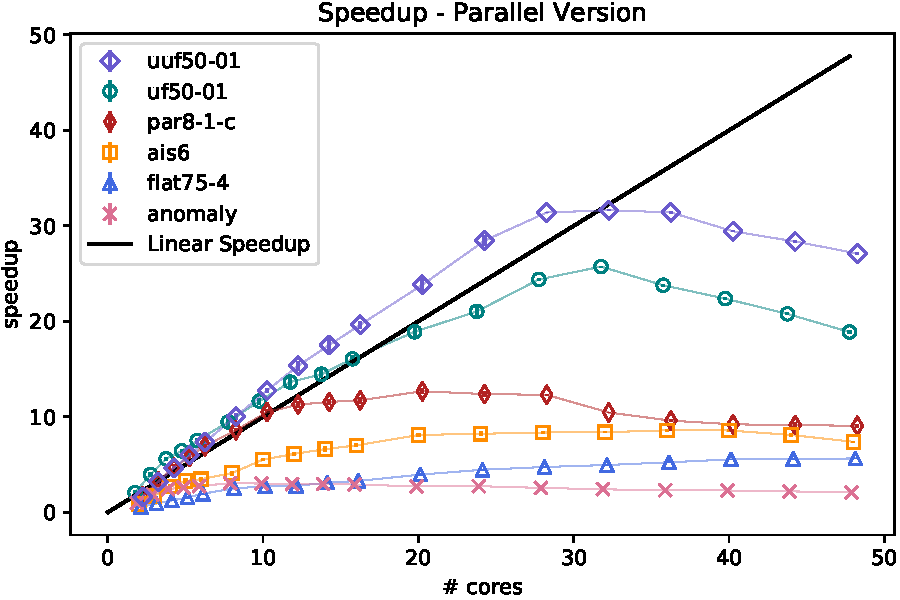
\includegraphics[width=\columnwidth]{figures/scaling_parallel_subset_dpll_scaling_tar.pdf}
    \caption{Average speedup of master slave parallel DPLL implementation compared to sequential DPLL.
    The 95\% confidence intervalls are shown as error bars but too small to be visible in some cases.
    \label{fig:dpll_parallel_speedup}}
\end{figure}
The speedup factor that we achieved heavily depends on the formula.
But it is not just the "size" of the problem or time required to solve a formula with the sequential algorithm that influences the speedup factor.
As shown in Table \ref{tab:cnfs_parallel} the formulas where we reached the highest speedup are not necessarily the ones with the largest number of variables, and therefore highest upper bound on the depth of the decision tree, or longest time to solve sequentially.
Note that the best speedup in this subset is actually achieved for the formula that is randomly generated (uf50-01).
For the random generated formula we can explain why the speedup goes down after about 32 cores:
After about 32 cores the master in our master-slave communication pattern starts to be a bottleneck and workers have to start waiting for pieces of work.
The overall average waiting time is shown in Figure \ref{fig:dpll_parallel_waiting}.
The waiting time is summed up over all the workers per solved formula and then averaged over different runs of the same formula.

The speedup is so small in some other cases because of the way the decision tree is traversed.
The sequential implementation deterministically does a depth-first search.
In this parallel version however we do not have any ordering guarantees.
It might happen that we were "close" to a solution but then solve some other partial models in a completely different part of the decision tree that might be unsatisfiable all together.
The size of the subtree where we will not find a solution depends on the structure of the formula.
This is also the explanation why we achieve super linear speedup in some other cases: there we are lucking and because of the traversal order find a solution faster than in the sequential traversal.

\begin{table}
    \centering
    \begin{tabular}{|l|c|c|}
        \hline
        formula & avg. runtime seq. DPLL [ms] & \# vars/clauses \\
        \hline
        \hline
        uf50-01 & 7890.9 +/-44.31 & 50/218\\
        \hline
        par8-1-c & 2185.0 +/- 32.88 & 64/254\\
        \hline
        ais6 &  2964.0 +/- 41.54 & 61/581\\
        \hline
        flat75-4 & 26284.6 +/- 172.65 & 225/840\\
        \hline
        par8-4- & 601.5 +/- 23.01 & 67/266\\
        \hline
        anomaly & 279.7 +/- 6.74 & 48/261\\
        \hline
    \end{tabular}
    \caption{Overview of benchmark subset formulas.}
    \label{tab:cnfs_parallel}
\end{table}

\begin{figure}
    \centering
    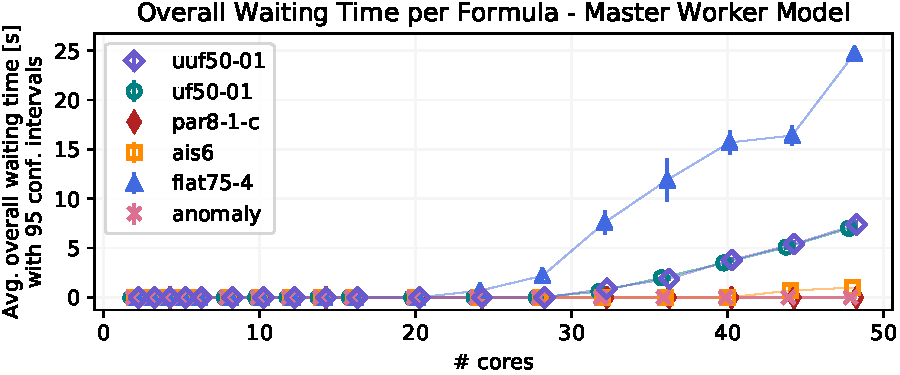
\includegraphics[width=\columnwidth]{figures/waiting_parallel_subset_dpll_scaling_tar.pdf}
    \caption{Average overall waiting time of workers per cnf in parallel version.
    All waiting times per worker are summed up.
    The 95\% confidence interval are shown as error bars.}
    \label{fig:dpll_parallel_waiting}
\end{figure}

\mypar{Stealing Scheduling}
Similar to the previous comparison, we compared the parallel work stealing algorithm to sequential DPLL.
\begin{figure}
  \centering
  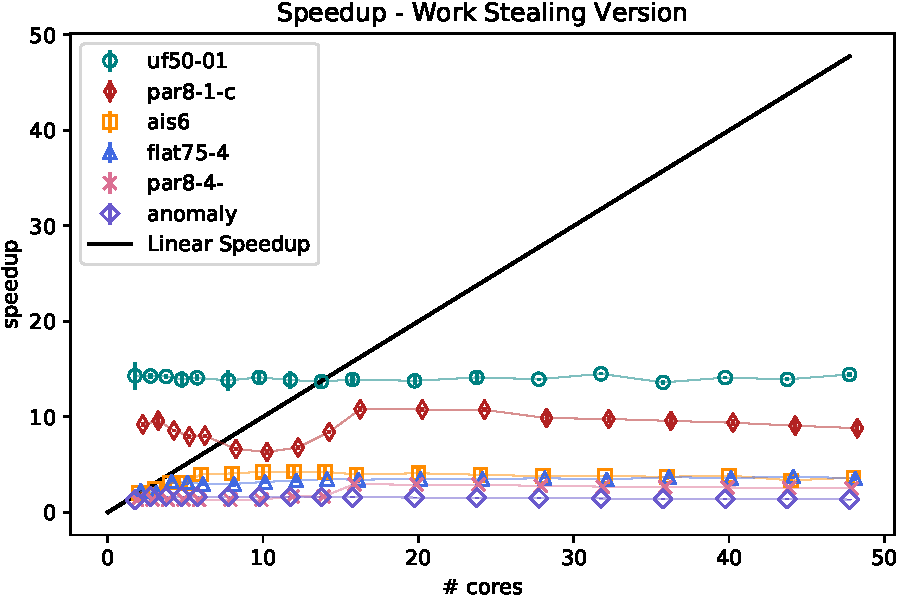
\includegraphics[width=\columnwidth]{figures/scaling_stealing_subset_dpll_scaling_tar.pdf}
  \caption{Speedup of work stealing parallel DPLL implementation compared to sequential DPLL.
  \label{fig:dpll_stealing_speedup}}
\end{figure}

The speedup that we achieve is shown in Figure \ref{fig:dpll_stealing_speedup}.
With this work stealing pattern we achieve quite high speedups for small numbers of cores but essentially do not gain from adding more cores after some limit.
The reason for this speedup is again the way how we traverse the decision tree.
In this pattern we do something that is similar to a breath first search globally and locally per node, the traversal order of the subtree is the same as in the sequential implementation, so depth first search.
That means that if the formula is satisfiable, we are guaranteed that some worker is working on the correct subtree already after the first decision and will never solve models of the other, wrong subtree.
This guarantee we do not have for the master slave pattern and we therefore beat the master slave pattern easily.

\section{Discussion}
In this section we will mention some of the things that we tried along the way but did not work out or we had to stop looking closer into because of time constraints.

\mypar{CDCL DPLL Hybrid Parallel Solver}
We have implemented a fully working CDCL solver.
If run sequentially it outperforms the DPLL solver on all of our 14 benchmark formulas.
Quite naturally we tried to plug that solver in at the workers.
The way we did that is the following:
\begin{itemize}
    \item First we run DPLL in parallel (it does not matter which of two communication patterns we pick).
    We only branch a certain number of times per worker.
    \item After that "branching limit" is reached we switch to CDCL and solve the whole subtree of the original decision tree locally.
    \item When that is done we either found a solution or again get a new model (either from the master or another worker) and solve it with CDCL.
\end{itemize}
With this hybrid approach we achieved really bad performance.
There are two reasons why.
Firstly we essentially cripple the CDCL solver by not giving him the full formula but only modified a part of it.
That means if we already decided something and then pass on that subproblem to the CDCL solver, the subproblem has not really a correlation to the original problem.
The problem that we solve with CDCL can be a completely different one and therefore a lot more difficult to solve then the original one.
Secondly, yet again we break something because of the way we split the work:
It might happen that all workers are busy solving some problem that is a lot more difficult than the actual problem and the subproblem that contains the correct solution is not solved by any worker at that point in time.
That means in the worst case we solve lots of partial models that are more difficult than the original problem, before we solve the correct problem and find the solution.

We ran everything we discussed in Section \ref{sec:exp} with this hybrid parallel solver for different branching limits.
We do not include any further information in this report because of space limitations.

\section{Future Work}
In this section we discuss possible extensions of our work.

\section{Conclusions}

Here you need to summarize what you did and why this is
important. {\em Do not take the abstract} and put it in the past
tense. Remember, now the reader has (hopefully) read the report, so it
is a very different situation from the abstract. Try to highlight
important results and say the things you really want to get across
such as high-level statements (e.g., we believe that .... is the right
approach to .... Even though we only considered x, the
.... technique should be applicable ....) You can also formulate next
steps if you want. Be brief. After the conclusions there are only the references.

% References should be produced using the bibtex program from suitable
% BiBTeX files (here: bibl_conf). The IEEEbib.bst bibliography
% style file from IEEE produces unsorted bibliography list.
% -------------------------------------------------------------------------
\bibliographystyle{IEEEbib}
\bibliography{bibl_conf}

\newpage
\section{Appendix}
This section contains additional information that is not strictly part of the report.

\begin{table}[h]
    \centering
    \begin{tabularx}{\columnwidth}{|l|X|}
        \hline
        File names & Description\\
        \hline
        \hline
        anomaly, medium & SAT-encoded blocks world planning problems\\
        \hline
        ais6, ais8 & SAT-encoded All-Interval Series problems\\
        \hline
        flat50-1, flat75-4 \\ flat 75-8 & SAT-encoded "Flat" Graph coloring problems (J. Coberson's flat graph generator is used\\
        \hline
        ii8a1 & Inductive inference, stem from a formulation of boolean function synthesis problems\\
        \hline
        par8-1-c, par8-5 & Instances for learning the paritiy function\\
        \hline
        uf50-01, uf75-01 & Uniform random 3-sat, satisfiable\\
        \hline
        uuf50-01, uf50-02 & Uniform random 3-sat, unsatisfiable\\
        \hline
    \end{tabularx}
    \caption{Description of benchmark problems.}
    \label{tab:benchmark_set}
\end{table}

\begin{figure}[h]
    \centering
    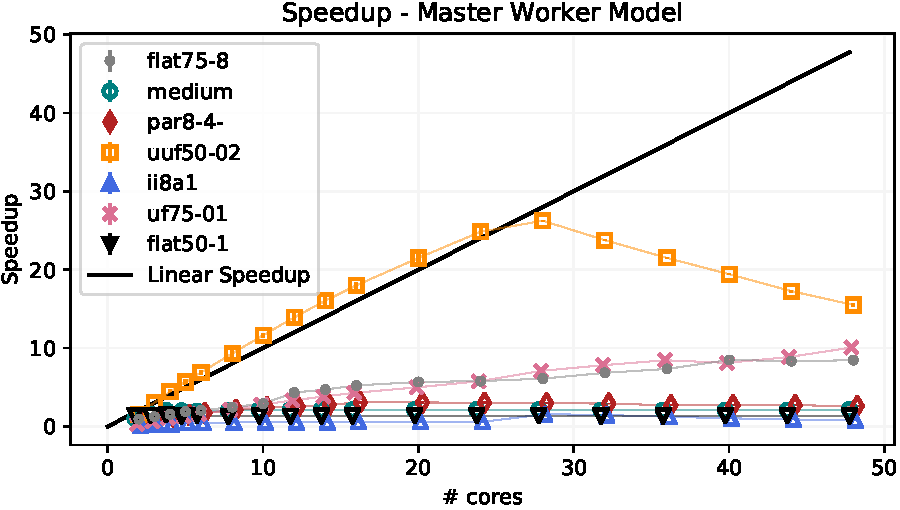
\includegraphics[width=\columnwidth]{figures/scaling_parallel_non_subset_dpll_scaling_tar.pdf}
    \caption{Average speedup of master slave parallel DPLL implementation compared to sequential DPLL.
    The 95\% confidence intervalls are shown as error bars but too small to be visible in some cases.
    Other subset.}
    \label{fig:dpll_parallel_speedup_non}
\end{figure}

\begin{figure}[h]
    \centering
    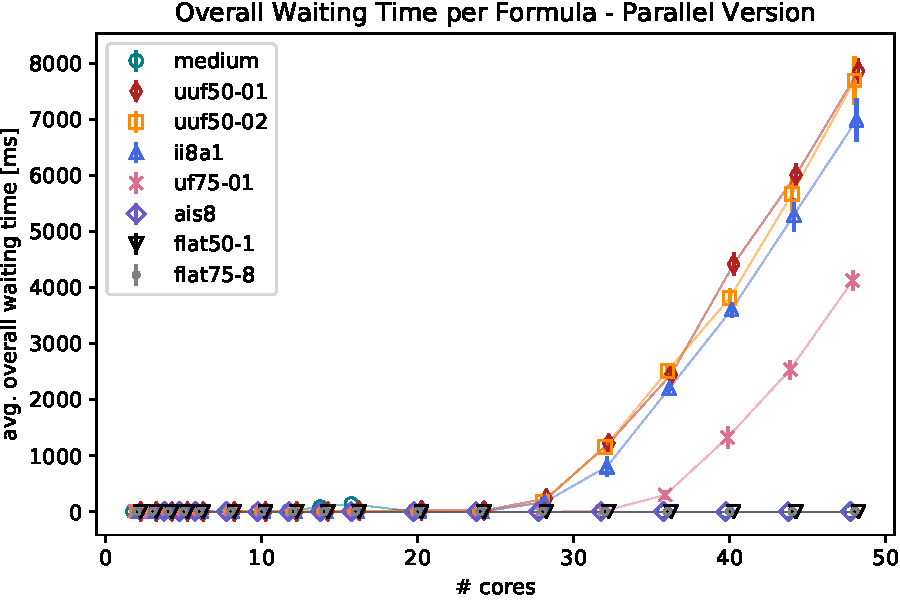
\includegraphics[width=\columnwidth]{figures/waiting_parallel_non_subset_dpll_scaling_tar.pdf}
    \caption{Average overall waiting time of workers per cnf in parallel version.
    All waiting times per worker are summed up.
    The 95\% confidence interval are shown as error bars.
    Other subset.}
    \label{fig:dpll_parallel_waiting_non}
\end{figure}

\begin{figure}[h]
    \centering
    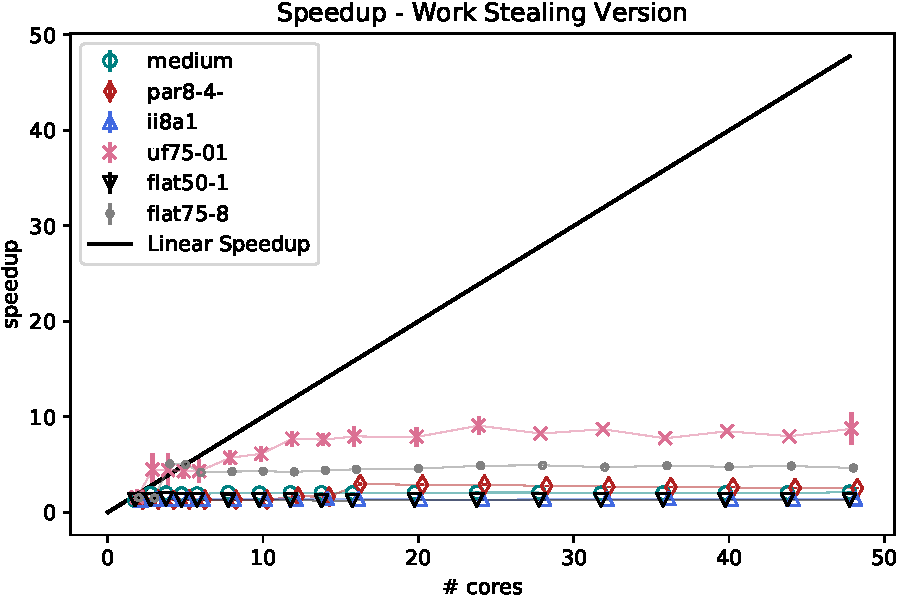
\includegraphics[width=\columnwidth]{figures/scaling_stealing_non_subset_dpll_scaling_tar.pdf}
    \caption{Speedup of work stealing parallel DPLL implementation compared to sequential DPLL.
    Other subset.}
    \label{fig:dpll_stealing_speedup_non}
\end{figure}

\begin{figure}[h]
    \centering
    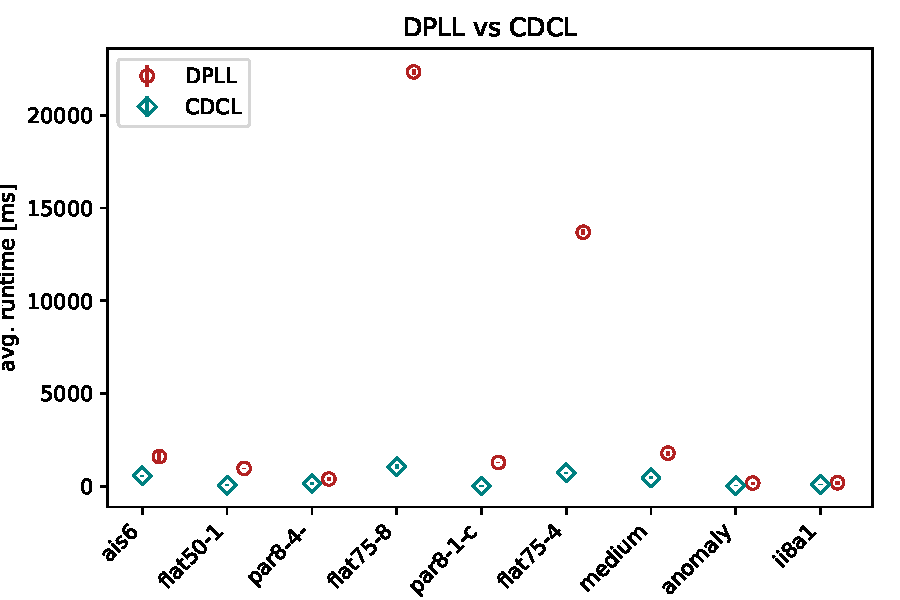
\includegraphics[width=\columnwidth]{figures/dpll_vs_cdcl.pdf}
    \caption{DPLL vs CDCL sequential runtime. Average runtime with 95\% confidence intervals.}
    \label{fig:dpll_stealing_speedup_non}
\end{figure}


\end{document}

